% Created 2015-06-01 Mon 16:22
\documentclass[11pt]{article}
\usepackage[utf8]{inputenc}
\usepackage[T1]{fontenc}
\usepackage{fixltx2e}
\usepackage{graphicx}
\usepackage{longtable}
\usepackage{float}
\usepackage{wrapfig}
\usepackage{rotating}
\usepackage[normalem]{ulem}
\usepackage{amsmath}
\usepackage{textcomp}
\usepackage{marvosym}
\usepackage{wasysym}
\usepackage{amssymb}
\usepackage{capt-of}
\usepackage{hyperref}
\tolerance=1000
\usepackage{minted}
\usepackage{color}
\usepackage{listings}
\usepackage{grffile}
\definecolor{mintedbackground}{rgb}{0.95,0.95,0.95}
\usepackage[inline]{enumitem}
\usepackage{xcolor}
\hypersetup{
colorlinks,
linkcolor={red!50!black},
citecolor={blue!50!black},
urlcolor={blue!80!black}
}
\usepackage{tikz,graphics,graphicx}
\usetikzlibrary{decorations.shapes,arrows,decorations.pathreplacing,decorations.pathmorphing,backgrounds}
\usetikzlibrary{decorations.pathmorphing}
\usetikzlibrary{shapes.geometric}
\usepackage{setspace}%% The linestretch
\singlespacing
\usepackage[format=hang,indention=0cm,singlelinecheck=true,justification=raggedright,labelfont={normalsize,bf},textfont={normalsize}]{caption} %
\usepackage{vmargin}
\setpapersize{A4}
\setmarginsrb{2.5cm}{1cm}% links, oben
{2.5cm}{2cm}% rechts, unten
{12pt}{30pt}% Kopf: Höhe, Abstand
{12pt}{30pt}% Fuß: Höhe, AB
\usepackage{upquote}
%  use straight quotes when printing a command in minted
\AtBeginDocument{%
\def\PYZsq{\textquotesingle}%
}
\setlength{\parindent}{0pt}
\setlength{\parskip}{\baselineskip}
\definecolor{mintedbackground}{rgb}{0.95,0.95,0.95}
\author{Alexander Jueterbock, Martin Jakt\thanks{University of Nordland, Norway}}
\date{\textbf{PhD course: High throughput sequencing of non-model organisms}}
\title{\textbf{Genome Assembly} (2015-06-04)}
\hypersetup{
 pdfkeywords={},
  pdfsubject={},
  pdfcreator={Emacs 24.3.1 (Org mode 8.3beta)}}
\begin{document}

\maketitle
\tableofcontents








After removing adapters and bad-quality reads, we are ready for \emph{de
novo} assembly of the sequenced genome libraries. The number of
available genomes is increasing, also for non-model species (for
marine species, see for example \href{http://cemeb.science.gu.se/research/imago-marine-genome-projects}{The IMAGO Marine Genome
projects}). Many analyses are only possible with a reference 
genome. Thus, \emph{de novo} assembly is a first important step for many
follow-up analyses, such as SNP-discovery for population-genomics or
differential-expression analysis based on RNAseq data.

\section{MIRA - assembler}
\label{sec-1}
The choice of \emph{de novo} sequence assemblers is wide (\href{http://en.wikibooks.org/wiki/Next_Generation_Sequencing_\%28NGS\%29/De_novo_assembly#Creating_a_dataset}{overview}). Some
of the better known open-source assemblers include \href{http://bioinf.spbau.ru/spades}{SPAdes}, \href{http://www.ebi.ac.uk/~zerbino/velvet/}{Velvet},
\href{http://soap.genomics.org.cn/soapdenovo.html}{SOAPdenovo}, and \href{http://sourceforge.net/projects/mira-assembler/}{MIRA}. Have a look on \href{http://gage.cbcb.umd.edu/index.html}{GAGE}, which compares the
performance of major assembly strategies.

We use \href{http://sourceforge.net/projects/mira-assembler/}{MIRA} in this tutorial because it can handle Ion Torrent
data. Please find its documentation \href{http://mira-assembler.sourceforge.net/docs/DefinitiveGuideToMIRA.pdf}{here}. Use the following command to
get an overview of the parameters: 

\begin{minted}[fontsize=\scriptsize,bgcolor=lightgray,linenos]{sh}
mira --help
\end{minted}

Before we start, we will create a folder that contains the data we
want to assemble:

\begin{minted}[fontsize=\scriptsize,bgcolor=lightgray,linenos]{sh}
mkdir GenomeAssembly
cd GenomeAssembly
mkdir data
\end{minted}

copy your quality-trimmed fastq file into the \texttt{data} directory with the command \texttt{cp}. 

The configurations for \texttt{mira} are specified in a so-called
\texttt{manifest} file. We won't have much time to play around with different
setting in this tutorial and will choose the most simple settings for
a \emph{de novo} genome assembly with Ion Torrent reads.


To create the manifest file in your \texttt{GenomeAssembly} directory, use
the command \texttt{touch}:

\begin{minted}[fontsize=\scriptsize,bgcolor=lightgray,linenos]{sh}
touch manifest.conf
\end{minted}

Now, to edit this file, we can use the command-line program
\texttt{nano}. This allows you to open and edit small text files from the command
line (no graphical user interface needed). To open the \texttt{manifest.conf}
file, just type:

\begin{minted}[fontsize=\scriptsize,bgcolor=lightgray,linenos]{sh}
nano manifest.conf
\end{minted}

Once you hit ENTER, \texttt{manifest.conf} will be opened. For now, it is
still empty. You can edit the content of the file by deleting and
adding text. At the bottom of the terminal window you see some
shortcuts for certain actions. For example \texttt{\textasciicircum{}O WriteOut} or 
\texttt{\textasciicircum{}X Exit}. The \texttt{\textasciicircum{}} indicates that you need to press CTRL+O or CTRL+X.

The \texttt{manifest.conf} file shall have the following content:

\begin{minted}[fontsize=\scriptsize,bgcolor=lightgray,linenos]{sh}
# Manifest file for de novo genome assembly with Ion Torrent single reads

project = IonTorrentDeNovoAssembly
job = denovo,genome,accurate

readgroup=UnpairedIonTorrentReadsFromHTSCourse2015
data = fastq::data/YOURINPUTFILE.fq
technology = iontor
\end{minted}

You can copy these lines and paste them into your file by pressing
SHIFT+CTRL+V. Change the name \texttt{YOURINPUTFILE.fq} to the name of the
fastq-file that contains your quality-trimmed reads. Then save the
file and exit with CTRL+O and CTRL+X.

That's all you need before you can start \texttt{mira} with:

\begin{minted}[fontsize=\scriptsize,bgcolor=lightgray,linenos]{sh}
nohup mira manifest.conf >log_assembly.txt &
\end{minted}

The analysis will take about 1 hour to finish.

\section{Results and assembly metrics}
\label{sec-2}
MIRA creates a directory named \texttt{IonTorrentDeNovoAssembly\_assembly} and several
subdirectories. We are primarily interested in the following two
subdirectories: 
\begin{itemize}
\item 1. \texttt{IonTorrentDeNovoAssembly\_d\_results}: this directory contains all the output
files of the assembly in different formats. Here we are specifically
interested in the following fasta files:
\begin{itemize}
\item \texttt{IonTorrentDeNovoAssembly\_out.padded.fasta}. This file contains the assembled contigs. Gaps are denoted by an asterisk.
\item \texttt{IonTorrentDeNovoAssembly\_out.unpadded.fasta}. This file also contains
the assembled contigs, but with positions containing gaps removed.
\item \texttt{LargeContigs\_out.fasta}. This file contains the longer contigs of
your assembly, which are of particular interest. To be included in
this file, a contig generally needs to be at least 500bp long and
must have a coverage of at least 1/3 of the average coverage.
\end{itemize}
\item 2. \texttt{IonTorrentDeNovoAssembly\_d\_info}: this directory contains files describing the properties of
the final assembly. We are particularly interested in:
\begin{itemize}
\item \texttt{IonTorrentDeNovoAssembly\_info\_assembly.txt}. This file contains
summary statistics and information about problematic areas in the
results. Here, 'Consensus bases with \href{http://www.bioinformatics.org/sms/iupac.html}{IUPAC}' refers to positions
that are not clearly 'A', 'C', 'T', or 'G', but where two or more
bases were equally likely. For example, 'R' refers to 'A or G', and
'K' refers to 'G or T'.
\item \texttt{IonTorrentDeNovoAssembly\_info\_contigstats.txt}. This file
contains statistics about the contigs themselves, their length,
average consensus quality, number of reads, maximum and average
coverage, average read length, number of A, C, G, T, N, X and gaps.
\end{itemize}
\end{itemize}


Search for the following information in \texttt{IonTorrentDeNovoAssembly\_info\_assembly.txt}:
\begin{itemize}
\item Number of contigs in the assembly
\item Maximum contig coverage
\item Largest contig
\item N50 contig size
\end{itemize}

Reminder on the N50 metric (see Fig. \ref{fig:N50}):


\begin{figure}[htb]
\centering
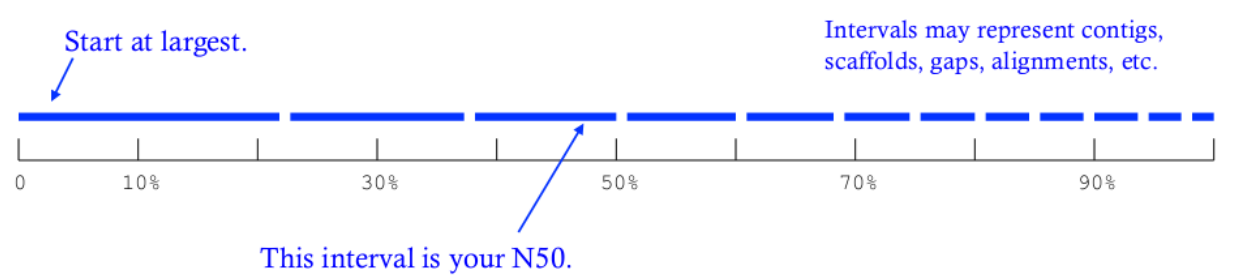
\includegraphics[width=11cm]{N50.png}
\caption{\label{fig:N50}From Kane, N.C.}
\end{figure}


N50 measures the median contig length in a set of sequences. The
larger it is, the closer your assembly gets to the real genome. N50 is
obtained by:
\begin{itemize}
\item 1. Sorting contigs in descending length order.
\item 2. Identifying the size of the contig above which the assembly contains at least 50\% of the
total length of all contigs.
\end{itemize}


We can use the program R to create histograms of the contig lengths
and coverages from the file
\texttt{IonTorrentDeNovoAssembly\_info\_contigstats.txt}. If you are in the
directory named \texttt{IonTorrentDeNovoAssembly\_assembly} (if you are not in
this directory, you can move to it with the \texttt{cd} command), you can
copy and paste the following commands into your terminal window to
plot histograms of the contig lengths and coverages:

\begin{minted}[fontsize=\scriptsize,bgcolor=lightgray,linenos]{sh}
rm Rplothistogram.r # Use this if the file Rplothistogram.r already exists.

cat >> Rplothistogram.r << 'EOF'
contigs <- read.table(
  file="IonTorrentDeNovoAssembly_d_info/IonTorrentDeNovoAssembly_info_contigstats.txt", 
  sep="\t", header=FALSE)

png(filename = "ContigLengths.png",
  width = 480, height = 480, units = "px", pointsize = 12,
  bg = "white")
hist(contigs$V2,main="Histogram of contig lengths",
  xlab="Contig length (bp)",ylab="Frequency",col="blue",breaks=100)
dev.off()

png(filename = "ContigCoverages.png",
  width = 480, height = 480, units = "px", pointsize = 12,
  bg = "white")
hist(log10(contigs$V6),main="Histogram of average log10 contig coverages",
  xlab="Average log10 contig coverage",ylab="Frequency",col="blue",breaks=100)
dev.off()

EOF

R CMD BATCH Rplothistogram.r
\end{minted}

Alternatively you can use R interactively by starting an R session
(just type \texttt{R} and return) and pasting the commands one by one into the
R session. In this case you can omit the \texttt{png(...)} and \texttt{dev.off()} commands;
these are used to create exportable images of plots (see below for more).

To open the figures, you can use the \texttt{eog} command, which is the
Eye of Gnome graphics viewer program:

\begin{minted}[fontsize=\scriptsize,bgcolor=lightgray,linenos]{sh}
eog ContigLengths.png
eog ContigCoverages.png
\end{minted}


Example histograms of contig lengths and coverages are shown in
Fig. \ref{fig:histcontlength} and \ref{fig:histcontcov}.

\clearpage

\begin{figure}[htb]
\centering
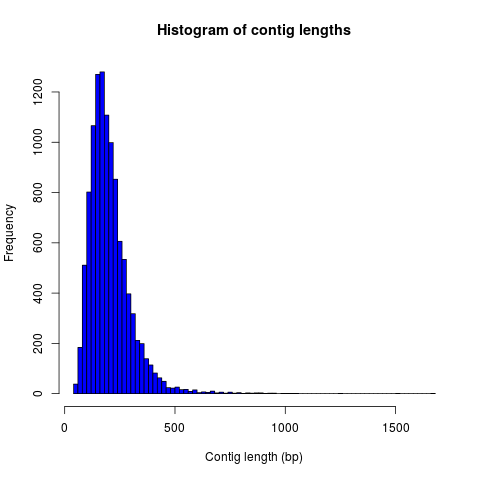
\includegraphics[width=8cm]{ContigLengths.png}
\caption{\label{fig:histcontlength}Histogram of contig lengths}
\end{figure}


\begin{figure}[htb]
\centering
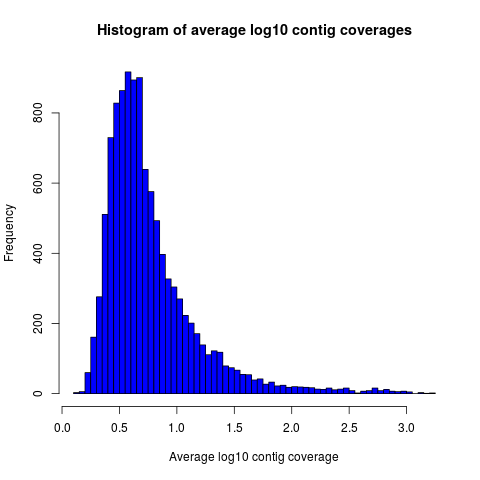
\includegraphics[width=8cm]{ContigCoverages.png}
\caption{\label{fig:histcontcov}Histogram of contig coverages}
\end{figure}





You can also extract the number of contigs>500bp and the sum of bases
in these contigs with R. Until now you have used R scripts with the \texttt{R
CMD BATCH} command, like the freshly created script \texttt{Rplothistogram.r}
above.

Instead of running \texttt{R} scripts from the shell command line, you can
also open an \texttt{R} command-line window where you can execute commands
directly. To start \texttt{R}, just type \texttt{R} in the terminal and hit
enter. All that comes after this command will be executed in the R
console. Lines preceded with a \texttt{\#}-sign will be ignored and serve only as
non-executed comments.

\begin{minted}[fontsize=\scriptsize,bgcolor=lightgray,linenos]{r}
R

# open the output file from MIRA
contigs <- read.table( 
file="IonTorrentDeNovoAssembly_d_info/IonTorrentDeNovoAssembly_info_contigstats.txt", 
  sep="\t", header=FALSE)

# Extract only those contigs that are longer than 500bp
contigs.above500 <- contigs[contigs[,2]>500,2]

# Count the number of contigs that are longer than 500bp
length(contigs.above500)
# Output for example: 156


# Count the number of bases in these contigs
sum(contigs.above500)
# Output for example 102297

# leave R again
q()
\end{minted}



MIRA does not only assemble your reads but it comes with a command
line tool named \texttt{miraconvert}, which allows you to extract contigs
based on, for example, contig length and coverage (see in the \href{http://mira-assembler.sourceforge.net/docs/DefinitiveGuideToMIRA.pdf}{MIRA
documentation} for further details and options).


\section{Automating the procedure}
\label{sec-3}
Using Unix based systems (including Linux) it is easy to automate procedures
through writing small shell scripts. These are very similar to running commands
from the command line; however, you also get the ability to make use of variables,
loops and conditionals which mean that you don't have to repetitively input commands
for every single file, but can do so once only.

The following script can be used to automate the trimming and assembly process
described in this and the previous lesson. To run the script simply enter the
directory containing your fastq files and:

\begin{minted}[fontsize=\scriptsize,bgcolor=lightgray,linenos]{sh}
./trimAndAssemble.sh *.fastq
\end{minted}

Assuming of course that the \texttt{trimAndAssemble.sh} script is located in the same directory.
For the course we will put this script into the \texttt{/usr/local/HTS\_scripts} folder, so
\texttt{/usr/local/HTS\_scripts *.fastq} is probably a better way to run it. However, if you
wish to modify the script you will need to copy it to your local directory first as
you will not have write access to common directories.

\begin{minted}[fontsize=\scriptsize,bgcolor=lightgray,linenos]{sh}
#!/bin/bash

## trim and quality control the sequences
## call for the original fastq files.

tr1Dir=trim1
tr2Dir=trim2

## this should create the directory if it doesn't exist
[ -d $tr1Dir ] || mkdir $tr1Dir
[ -d $tr2Dir ] || mkdir $tr2Dir

for f in $@; do
    f2=`echo $f | sed -r 's/\.fastq$|\.fq$/_trimmed\.fq/'`
    ## f2 will be the name of the first output file
    f2d=$tr1Dir"/"$f2
    ## lets run trim_galore on $f with output to the $tr1Dir directory
    ## only run if the output file doesn't exist
    [ -f $f2d ] || trim_galore -o $tr1Dir -a CCATCTCATCCCTGCGTGTCTCCGACTCAG --stringency 3 $f
    ## trim_galore will change the name of the file  
    ## as above. Check for the existence of the file
    if [ -f $f2d ] ; then
        echo " $f2d successfully created"
    else
        echo "Failed to created $f2d"
        echo "Will exit here"
        exit 1
    fi
    ## get the next output name
    f3=`echo $f2 | sed -r 's/\.fq$/_trimmed\.fq/'`
    f3d=$tr2Dir"/"$f3
    ## then run trim_galore again, this time to tr2Dir
    [ -f $f3d ] || trim_galore -o $tr2Dir \
        -a CCACTACGCCTCCGCTTTCCTCTCTATGGGCAGTCGGTGAT \
        --stringency 3 $f2d

    if [ -f $f3d ] ; then
        echo " $f3d successfully created"
    else
        echo "Failed to created $f3d"
        echo "Will exit here"
        exit 2
    fi
    ## then we can run fastqc if we wish, or we can just go ahead and run
    ## the assembly.. 

    ## we could also run the fastx_collapser to combine and count all identical reads, but
    ## let's not bother for now as this doesn't modify any of the files.

    ##### Running the assembly process. This requires setting up some directories for each
    ##### file and then starting the process to run in the background, using nohup.
    ##### note that running all of them, may use too many processors or too much memory, but let's give
    ## it a try anyway..

    ## first make a directory for the file..
    assDir=`echo $f | sed -r 's/\.fastq|\.fq//'`
    assDir=$assDir"_ass/"
    dataDir=$assDir"data"
    mkdir -p $dataDir
    mv $f3d $dataDir
    ## then make the manifest file..
    manfile=$assDir"manifest.conf"
    touch $manfile
    cat >> $manfile <<EOF
project = IonTorrentDeNovoAssembly
job = denovo,genome,accurate
readgroup=UnpairedIonTorrentReadsFromHTSCourse2015
data = fastq::data/*.fq
technology = iontor
EOF
    cd $assDir
    nohup mira manifest.conf > log_assembly.txt &
    cd ..
done
\end{minted}

Try to understand how this script works; to experiment with it you
can replace calls to run time consuming programs like \texttt{trim\_galore} with calls
to \texttt{echo} the commands, eg:

\begin{minted}[fontsize=\scriptsize,bgcolor=lightgray,linenos]{sh}
echo "trim_galore -o $tr1Dir -a CCAATACCA --stringency 3 $f"
\end{minted}

This will allow you to make sure that the script calls the various
programs correctly before you actually go ahead and run them.

Note that this script assumes that the current working directory contains a set
of fastq for which we wish to construct independent assemblies. If you wished
to make a unified assembly you can (probably) simply concatenate all the files
into a single file (\texttt{cat *.fastq > all\_files.fastq}) and specify this single
file. Note that this will only works if all the sequences have unique sequence
identifiers; this should generally be the case but will depend on the sequencing
setup used. If in doubt you should check; this can be done with a few lines
of Perl.

Using a script to automate the mapping procedure isn't just a good thing
because you get to spend less time typing commands into a terminal window.
The main advantages of running the procedure with a script are instead:

\begin{itemize}
\item You are less likely to make mistakes when running repeated tasks, and
you can be sure that every sequence file has been treated in the same way.

\item You have a record of how the mapping was carried out making it easier to
perform exactly the same procedure at some point in the future.
\end{itemize}

These two points are especially important if your project will be generating
data over a longer period of time that you need to continuously incorporate
into some analysis. In such a case you should also minimise the number
of arguments that are passed to the scripts running the analysis and for
even bigger projects you might set the script such that it automatically updates
a database describing your analytical pipeline.

\section{Next steps to consider}
\label{sec-4}

Hint: to identify the proportion of contigs that are protein-coding
and the proportion that may result from bacterial contamination, you
can use the Basic Local Alignment Search Tool (\href{http://blast.ncbi.nlm.nih.gov/Blast.cgi}{BLAST}) to align the
contigs to databases with known genes and proteins.

MIRA assembles the reads to so-called contigs, which are based on
overlapping sequences. Contigs can be joined with mate-pair libraries
into longer fragments (often referred to as scaffolds, which are
basically contigs that were connected by gaps, see figure below). MIRA
does not perform scaffolding. This can be done with the stand-alone
\href{http://www.baseclear.com/genomics/bioinformatics/basetools/SSPACE}{SSPACE} software.


\begin{center}
\begin{figure}[htb]
\setlength{\belowcaptionskip}{-1cm}
\scalebox{0.5}{
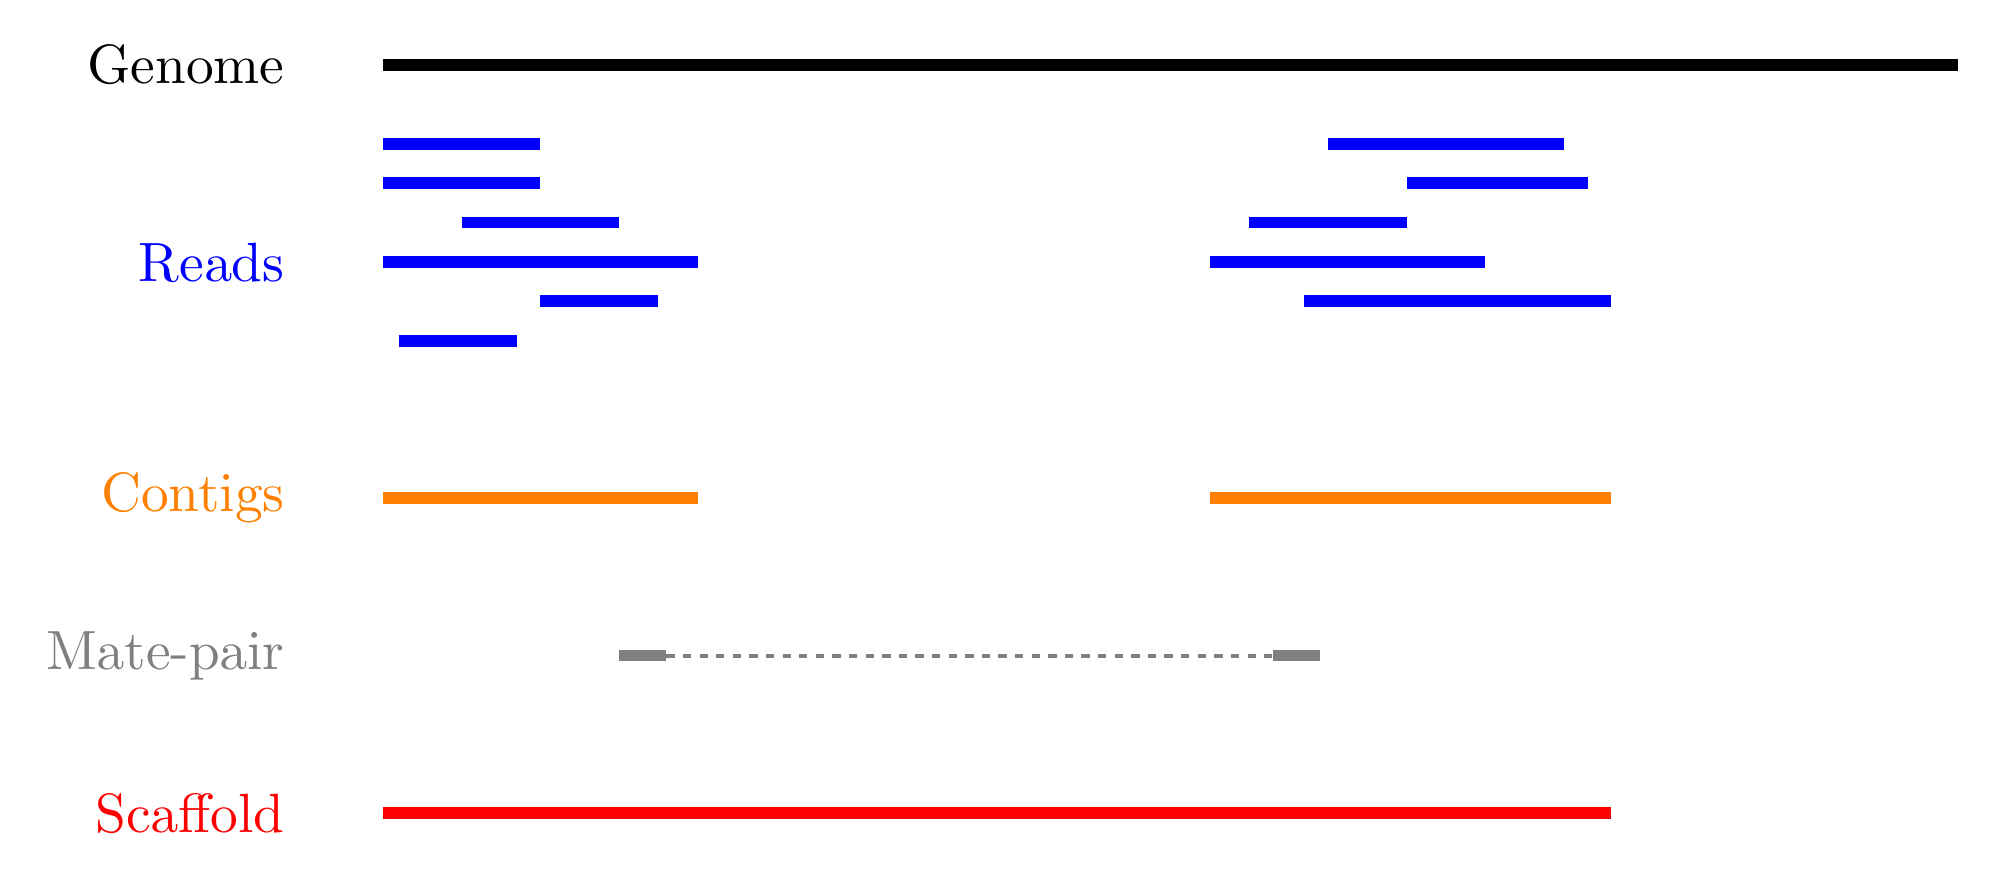
\begin{tikzpicture}

\node [anchor=east, scale=2] at (-1cm, 0.5cm) {Genome};
\node [anchor=east, scale=2,color=blue] at (-1cm, -2cm) {Reads};
\node [anchor=east, scale=2,color=orange] at (-1cm, -5cm) {Contigs};
\node [anchor=east, scale=2,color=gray] at (-1cm, -7cm) {Mate-pair};
\node [anchor=east, scale=2,color=red] at (-1cm, -9cm) {Scaffold};

\draw [line width=0.15cm, anchor=west] (0cm,0.5cm) -- (20cm,0.5cm);


\draw [line width=0.15cm, anchor=west,color=blue] (0cm,-0.5cm) -- (2cm,-0.5cm);
\draw [line width=0.15cm, anchor=west,color=blue] (0cm,-1cm) -- (2cm,-1.cm);
\draw [line width=0.15cm, anchor=west,color=blue] (1cm,-1.5cm) -- (3cm,-1.5cm);
\draw [line width=0.15cm, anchor=west,color=blue] (0cm,-2cm) -- (4cm,-2cm);
\draw [line width=0.15cm, anchor=west,color=blue] (2cm,-2.5cm) -- (3.5cm,-2.5cm);
\draw [line width=0.15cm, anchor=west,color=blue] (0.2cm,-3cm) -- (1.7cm,-3cm);

\draw [line width=0.15cm, anchor=west,color=blue] (12cm,-0.5cm) -- (15cm,-0.5cm);
\draw [line width=0.15cm, anchor=west,color=blue] (13cm,-1cm) -- (15.3cm,-1cm);
\draw [line width=0.15cm, anchor=west,color=blue] (11cm,-1.5cm) -- (13cm,-1.5cm);
\draw [line width=0.15cm, anchor=west,color=blue] (10.5cm,-2cm) -- (14cm,-2cm);
\draw [line width=0.15cm, anchor=west,color=blue] (11.7cm,-2.5cm) -- (15.6cm,-2.5cm);

\draw [line width=0.15cm, anchor=west,color=orange] (0cm,-5cm) -- (4cm,-5cm);
\draw [line width=0.15cm, anchor=west,color=orange] (10.5cm,-5cm) -- (15.6cm,-5cm);

\draw [line width=0.15cm, anchor=west,color=gray] (3cm,-7cm) -- (3.6cm,-7cm);
\draw [line width=0.05cm, dashed, anchor=west,color=gray] (3.6cm,-7cm) -- (11.3cm,-7cm);
\draw [line width=0.15cm, anchor=west,color=gray] (11.3cm,-7cm) -- (11.9cm,-7cm);

\draw [line width=0.15cm, anchor=west,color=red] (0cm,-9cm) -- (15.6cm,-9cm);

\end{tikzpicture}
} 
\end{figure}
\end{center}

\section{Counting codons}
\label{sec-5}

In this course you will have hopefully obtained a fair amount of genomic sequence and
been able to assemble this into a set of contigs. However, unless your DNA source
has a remarkably small genome (or is mitochondrial) you will not have been able to
assemble anything resembling a complete genome. What you will have obtained is a sampling
of the genomic sequence of your source organism. Today, that isn't likely to provide you
with a great deal of new biological insights since so much has already been sequenced.
However, a few years ago, the sequence you will have obtained during this course would
have required a great deal of resources and consequently much effort would also have
been spent to extract biological information from the sequence.
It is not immediately obvious what sort of information we can obtain from the sequence,
but the following spring to mind:

\begin{itemize}
\item Nucleotide composition. This varies between species, with species that are exposed
to high temperatures (e.g. \emph{Thermus aquaticus}) will tend to be very G/C rich.

\item CpG dinucleotide composition, and in particular in relation to the G/C frequencies.
The presence of regions of atypically high (CgG : G/C) ratios (i.e. CpG islands)
are indicative of CpG methylation.

\item K-mer frequencies, to detect over-represented sequences and to define random models
for genomic sequences (useful when trying to identify sequences over-represented in
specific regions).

\item Detection of known and novel repeat sequences.

\item Quantification of the coding potential of the genome. This is easier if done in combination
with RNA sequences, or in species which do not have introns. However, it is possible to
make inferences from the distribution of open reading frame (ORF) lengths, or better yet, by
running tblastx to look for regions that encode peptide sequences
that are likely to be functional.

\item Quantification of codon usage. Different species tend to use different amino acid encoding
and this can be observed from the frequencies of codon usage.
\end{itemize}

For your own work, you probably have specific questions that you wish to answer, and you
probably have little interest in the questions addressed above. It's also fairly likely that
these questions have already been addressed for your species of interest. However, for an
organism which has not already been extensively sequenced you really should quantify these types
of parameters. If you're lucky your organism may be an outlier of some sort, and if not it at
least provides you with a characterisation of the basal properties of the genome sequence and this
is useful to have for more detailed analyses.

For this course we have prepared a small Perl script that counts codon frequencies in DNA
sequences. The script reads in data from Fasta sequence files and counts codons in all 6 frames. 
As the majority of the sequence is likely to not encode peptide sequences,
the script performs separate counts for ORFs of different sizes (specified within the script
itself). The resulting codon counts (or frequencies) depend both on the amino acid content
of the encoded peptides and on the bias for specific codon usage per amino acid. 
It would be better to quantify these two seperately and the script can be fairly easily modified
to do this. The script has not been optimised for speed; tests on last year's course data suggests
it will require no more than a few minutes to run, and this means it's not worthwhile to spend
time to increase its performance. However, for larger sequencing projects, it would probably be
worthwhile to get something faster, either by using somebody else's program (there are bound
to be lots around), by modifying the Perl script or rewriting it in a compiled language like C
or C++ (not really that difficult).

We will make the script available in \texttt{/usr/local/HTS\_scripts}, or if you're so inclined
you can copy the following code into a text editor (like in the old days).

\begin{minted}[fontsize=\scriptsize,bgcolor=lightgray,linenos]{perl}
#!/usr/bin/perl -w
use strict;

## read a fasta file and output codon usages within ORFs of different minimum
## sizes. 

## in this I use substr to do most of the work. That's probably pretty terrible
## a better way would probably be to use unpack.. We can do something like
## @nucs = unpack( 'a1' x length($seq), $seq )
## @nucs = unpack( 'C*', seq)
## 
## which should speed things up by a large amount.

my $seqFile = shift @ARGV;

## the minium sizes of ORFs
## in codon counts.
my @minSizes = (10, 20, 40, 80, 160, 320, 640);

## for the sake of simplicity, this script will make use of a
## global %codonUsage hash. This is generally speaking a bad idea
## but it's easy to implement

my %stopCodons = ('TAA' => 1, 'TAG' => 2, 'TGA' => 3);
my %codonTable = generateCodonTable();

my %codonCounts = (); 
## then we can use if(defined to check for a stop codon)

## read the seqfile and get the codon counts.
open(IN, $seqFile) || die "unable to open $seqFile $!\n";

my $seqId = "";
my $seq = "";
while(<IN>){
    chomp;
    if($_ =~ /^>(\S+)/){
        $seqId = $1;  
        if(length($seq)){
            countSeqCodons($seq);
        }
        $seq = "";
        next;
    }
    $seq .= uc($_);  ## assumes that the sequence is clean
}
if(length($seq)){ countSeqCodons($seq) }

print "\t";
for my $c(@minSizes){
    print "\t", $c;
}
print "\n";

for my $i(sort keys %codonTable){
    print $codonTable{$i}, "\t", $i;
    for my $c(@minSizes){
        print "\t";
        if(defined($codonCounts{$c}{$codonTable{$i}})){
            print $codonCounts{$c}{$codonTable{$i}};
        }
    }
    print "\n";
}
\end{minted}

\begin{minted}[fontsize=\scriptsize,bgcolor=lightgray,linenos]{perl}
###################################################################################
## Functions or subroutines.
## These are called within the code by their name followed by a pair of brackets
## containing the arguments to the function, eg:
##
## function_name( arg1, arg2, arg3 );
##
## or with no arguments:
## function_name();
##
## the values of the variables are copied to the function where they are referred to
## by an array called @_
##
## modifying the values of variables within @_ does not modify the value of the argument
## passed to the function. However, we can pass a reference to a variable to functions
## and this allows the function to modify the values of the argument variables. To pass
## a value as a refence, we put a \ in front of it. Eg. 
##
## function_name( \%hash )
##
## to pass a hash as an reference (see below). This can also be used to pass several
## variable length arguments to the function.


sub countSeqCodons {
    ## this copies the value of the first argument to the variable $s. This is completely
    ## unnecessary, but it is easier to read and write $s than $_[0], and this makes it
    ## easier to avoid making stupid mistakes.
    my $s = $_[0];
    my $rs = revComplement($s);
    for my $f(0..2){
        my @sc = findOrfs($s, $f);
        my @rsc = findOrfs($rs, $f);
        ## these two are the same, 
        countCodons(@sc);
        countCodons(@rsc);   ## these could be passed by reference which might speed things up
    }
}

sub countCodons {
    ## $l refers to the length of a sub ORF
    my $l = 0;
    my %codonUsage = ();
    for my $i(@_){
        $codonUsage{$i}++;  ## this will include stop codon usage
        ++$l;
        ## stop codons have been assigned negative values so we can check for the end of an
        ## ORF by:
        if($i < 0){
            incrementCodonCounts($l, \%codonUsage);
            %codonUsage = ();
            $l = 0;
        }
    }
    incrementCodonCounts($l, \%codonUsage);
}

sub incrementCodonCounts {
    my $l = shift(@_);
    my %counts = %{$_[0]};  ## this should be a reference to the hash calculated previously
    my $i = 0;
    while($i < $#minSizes && $l > $minSizes[$i]){
        ++$i;
    }
    for my $c( keys %counts ){
        $codonCounts{ $minSizes[$i] }{ $c } += $counts{$c};
    }
}
\end{minted}

\begin{minted}[fontsize=\scriptsize,bgcolor=lightgray,linenos]{perl}
## make a hash of codon to number so
## that we can represent a sequence of codons as an array
## of numbers. This doesn't actually save any memory, or speed
## up the process, but it does make it easier to read and write
## the code.
sub generateCodonTable {
    my @nt = ('A', 'C', 'G', 'T');
    my %codonTable = ();
    my $i = 1;
    for my $n1(@nt){
        for my $n2(@nt){
            for my $n3(@nt){
                my $codon = $n1.$n2.$n3;
                $codonTable{$codon} = $i++;
                if(defined($stopCodons{$codon})){
                    $codonTable{$codon} = -$codonTable{$codon};
                }
            }
        }
    }
    return( %codonTable );
}

## makes use of the global
## codonTable and stopCodons
sub findOrfs {
    my($s, $frame) = @_;
    my @orc;  ## numerical code, use 0 for stop codons or others
    if($frame < 0){
        ## we die here, because rev complementing here would mean we do it 
        ## three times rather than once..
        die "This function only accepts positive frames. RevComplement elsewhere\n";
    }
    my $b = $frame;
    while($b <= (length($s) - 3)){
        my $ss = substr($s, $b, 3);
        my $c = 0;
        if(!defined($codonTable{$ss})){
            print STDERR "Unknown codon $ss\n";
        }
        if( defined($codonTable{$ss}) ){
            $c = $codonTable{$ss};
        }
        push @orc, $c;
        $b += 3;
    }
    return(@orc)
}

sub revComplement {
    my $s = $_[0];
    my $rs = $s;
    my %comp = ('A' => 'T', 'C' => 'G', 'G' => 'C', 'T' => 'A',
                'R' => 'Y', 'Y' => 'R', 'S' => 'S', 'W' => 'W',
                'K' => 'M', 'M' => 'K', 'B'=>'V', 'V' => 'B', 'D' => 'H',
                'H' => 'T', 'N' => 'N');
    ## that can be written faster with qw() and implicit conversion of an array to a hash.
    for(my $i=0; $i < length($s); $i++){
        substr($rs, length($rs)-$i-1, 1) = $comp{substr($s, $i, 1)};
        ## which will complain loudly if we have non standard codes
    }
    return($rs);
}
\end{minted}

To run the script, merely do \texttt{./count\_codons.pl seq.fa > counts.txt} where, \texttt{seq.fa} is the fasta
file containing the sequences you wish to cound. The script will print a table of codon counts
to \texttt{counts.txt} for ORFs of different length ranges. 
This can be imported and analysed within R. To visualise the tendencies of the codon usages I
have combined this data set with data from a database of codon usage in a wide range of
species (\url{ftp://ftp.kazusa.or.jp/pub/codon/current/}), and used the frequencies to perform a
principal components analysis (PCA) Fig. \ref{fig:codonpca}: 

\begin{figure}[htb]
\centering
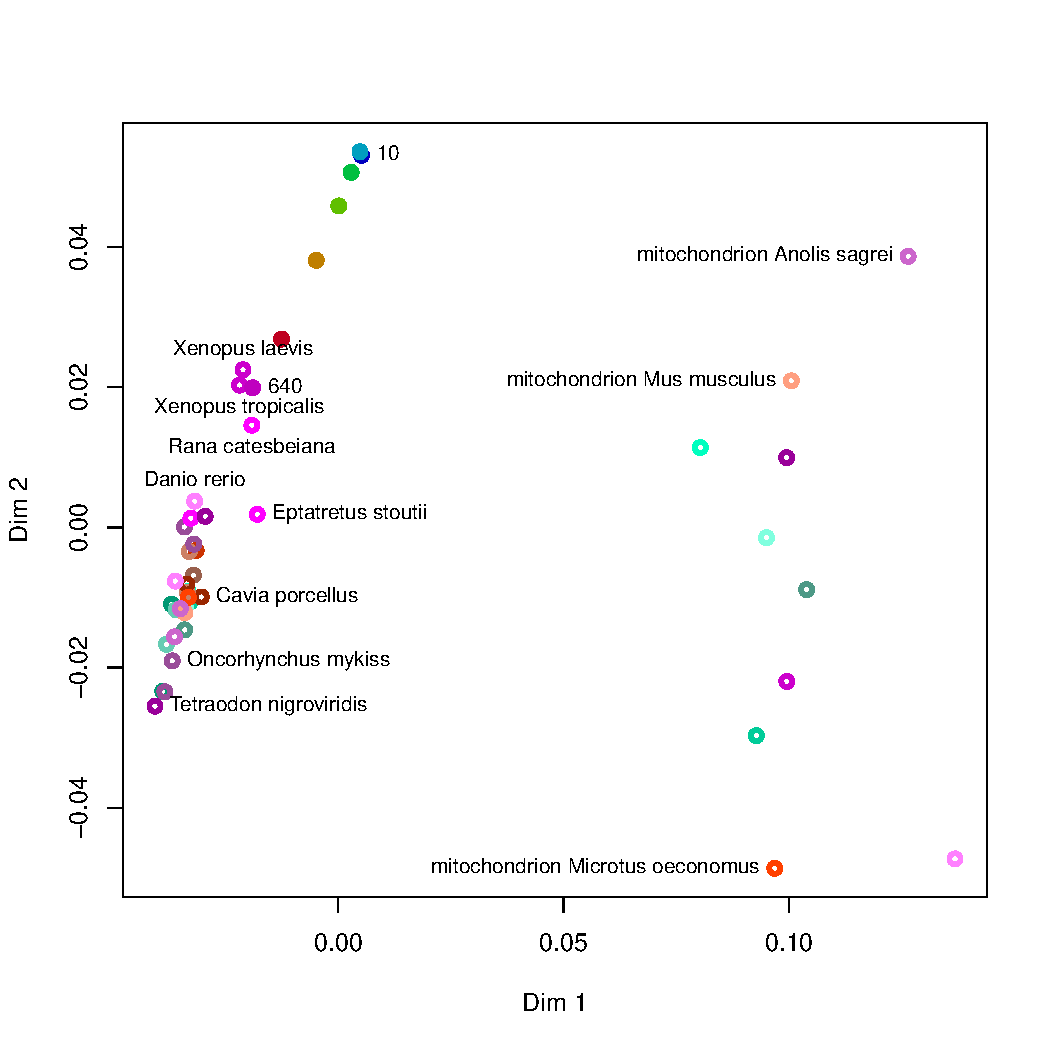
\includegraphics[width=14cm]{CodonFrequency_PCA.pdf}
\caption{\label{fig:codonpca}Principal components analysis of codon usage in vertebrate species. Open circles represent data from the published database. Closed circles represent data from sequences produced at last year's course; the numbers (and colours) indicate the ORF lengths used to compile the codon frequencies. The first dimension of the PCA (x-axis) clearly segregates mitochondrial (right) and genome (left) encoded proteins.}
\end{figure}


To simplify the analysis I have restricted the PCA to vertebrate species: the majority of the
species in the database are bacterial, and there are also a large number of invertebrate species and
trying to visualise all of them at the same time is kind of messy. The analysis does include 
data from mitochondrial sequences
and these are clearly segregated from genomic encoded ones. Note how the points representing
the unknown sample become more similar to previously determined frequencies as the ORF length
increases.

To perform this analysis, I did write another small Perl script to parse codon counts from
the database files, and a bit of R code to have a look at the data. These codes will also
be made available for you in \texttt{/usr/local/HTS\_scripts}.
Emacs 24.3.1 (Org mode 8.3beta)
\end{document}